% ===== 04-gradient-descent =====
\section*{Gradient Descent}

\subsection*{Batch Gradient Descent}
\textbf{Batch} = every step uses \emph{all} $N$ training examples to compute the gradient.

Start with some weights $\mathbf{w}$, usually all zeros. Then repeat:
\begin{itemize}
  \item Look around the current point and find the steepest \emph{downhill} direction.
  \item Take a small step in that direction.
  \item Stop when the error stops going down.
\end{itemize}

{\centering
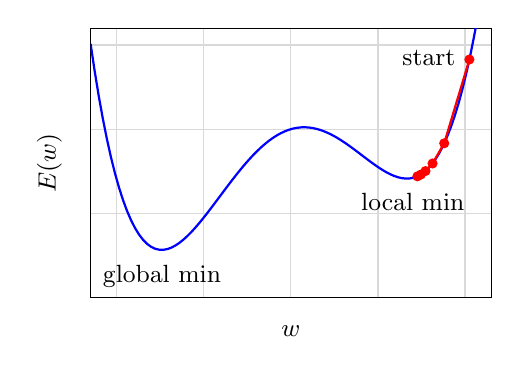
\begin{tikzpicture}
\begin{axis}[
    width=0.55\linewidth, height=5cm,
    xmin=-2.3, xmax=2.3, ymin=0, ymax=3.2,
    enlargelimits=false,
    grid=major, grid style={gray!30}, major tick length=0pt,
    xlabel={$w$}, ylabel={$E(w)$},
    tick label style={font=\small}, label style={font=\small},
    xticklabels={}, yticklabels={}
]
\addplot[thick, blue, domain=-2.3:2.3, samples=100] {0.25*x^4 - x^2 + 0.3*x + 2};
\addplot[red, thick, mark=*, mark size=1.4pt] coordinates {
    (2.050,2.828) (1.761,1.832) (1.627,1.592) (1.546,1.502) (1.492,1.460) (1.453,1.439)
};
\node[font=\small, anchor=east] at (axis cs:2.0,2.85) {start};
\node[font=\small, anchor=north] at (axis cs:1.4,1.35) {local min};
\node[font=\small, anchor=north] at (axis cs:-1.48,0.5) {global min};
\end{axis}
\end{tikzpicture}
\par}

\begin{itemize}
  \item The step size is called the \textbf{learning rate}: too big overshoots, too small is slow.
  \item Depending on where you start, you can end up in a \textbf{local minimum} instead of the global one.
  \item For linear regression, the error is a quadratic function, so there is only one minimum.
\end{itemize}

\textbf{Another view:} each step changes $\mathbf{w}$, which changes the line. Starting from $\mathbf{w} = \mathbf{0}$ (a flat line at 0), every step fits the data a little better until it converges.

{\centering
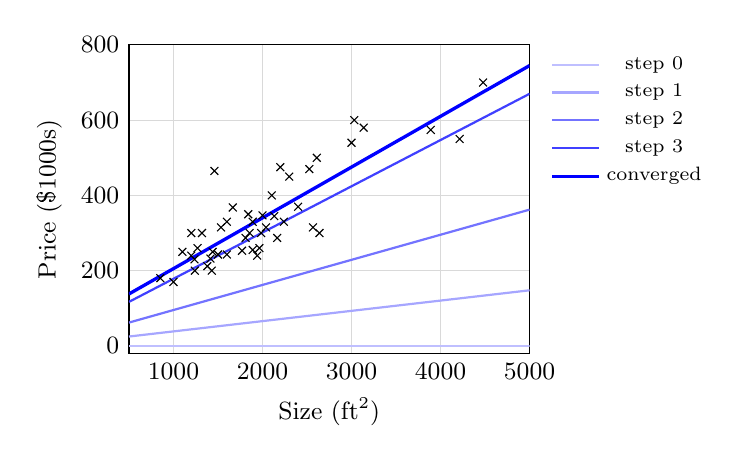
\begin{tikzpicture}
\begin{axis}[
    width=0.55\linewidth, height=5.5cm,
    xmin=500, xmax=5000, ymin=-20, ymax=800,
    enlargelimits=false,
    grid=major, grid style={gray!30}, major tick length=0pt,
    xlabel={Size (ft$^2$)}, ylabel={Price (\$1000s)},
    tick label style={font=\small}, label style={font=\small},
    xticklabel style={/pgf/number format/1000 sep={}},
    legend pos=outer north east, legend style={font=\scriptsize, draw=none, fill=white, fill opacity=0.8, text opacity=1}
]
\addplot[only marks, mark=x, mark size=2pt, black, forget plot] coordinates {
(852,180)(1000,170)(1100,250)(1200,300)(1200,240)(1236,230)(1240,200)(1270,260)
(1320,300)(1380,212)(1415,232)(1440,250)(1430,200)(1460,465)(1500,243)(1534,315)
(1600,330)(1600,243)(1666,368)(1770,253)(1810,287)(1840,350)(1855,300)(1890,330)
(1890,255)(1940,240)(1965,260)(1985,300)(2000,347)(2040,315)(2104,400)(2132,345)
(2165,287)(2200,475)(2240,330)(2300,450)(2400,370)(2526,470)(2567,315)(2610,500)
(2640,300)(3000,540)(3031,600)(3137,580)(3890,574)(4215,550)(4478,700)
};
\addplot[blue!25, thick, domain=500:5000, samples=2] {0};
\addlegendentry{step 0}
\addplot[blue!35, thick, domain=500:5000, samples=2] {11.3 + 0.0273*x};
\addlegendentry{step 1}
\addplot[blue!55, thick, domain=500:5000, samples=2] {28.7 + 0.0667*x};
\addlegendentry{step 2}
\addplot[blue!75, thick, domain=500:5000, samples=2] {55.6 + 0.1229*x};
\addlegendentry{step 3}
\addplot[blue, very thick, domain=500:5000, samples=2] {70.6 + 0.1349*x};
\addlegendentry{converged}
\end{axis}
\end{tikzpicture}
\par}

\textbf{Update rule.} Repeat until convergence, for every $d = 0, 1, \dots, D$:
\[
w_d := w_d - \eta \, \frac{\partial E(\mathbf{w})}{\partial w_d}
\]
\begin{itemize}
  \item $:=$ means assignment (overwrite $w_d$ with the right side).
  \item $\eta$: learning rate. The partial derivative points uphill, so we subtract it.
\end{itemize}

\textbf{Computing the derivative.} Start with one training example $(\mathbf{x}, t)$. Write $y = y(\mathbf{x},\mathbf{w})$ for short.
\begin{align*}
\frac{\partial}{\partial w_d}\, \frac{1}{2}(y - t)^2
&= (y - t) \cdot \frac{\partial}{\partial w_d}(y - t)
  \qquad \text{(chain rule; the 2 cancels the $\tfrac12$)} \\
&= (y - t) \cdot \frac{\partial}{\partial w_d}\big(w_0 x_0 + \dots + w_d x_d + \dots + w_D x_D - t\big) \\
&= (y - t)\, x_d
  \qquad \text{(only $w_d x_d$ depends on $w_d$)}
\end{align*}

For all $N$ examples, sum (the derivative of a sum is the sum of the derivatives):
\[
\frac{\partial E(\mathbf{w})}{\partial w_d} = \sum_{n=1}^{N} \big(y(\mathbf{x}_n,\mathbf{w}) - t_n\big)\, x_{n,d}
\]

\textbf{Final algorithm.} Repeat until convergence, for every $d$:
\[
w_d := w_d - \eta \sum_{n=1}^{N}
\underbrace{\big(y(\mathbf{x}_n,\mathbf{w}) - t_n\big)}_{\text{error on example } n}\,
\underbrace{x_{n,d}}_{\text{feature } d}
\]
\begin{itemize}
  \item The $\sum_{n=1}^{N}$ is what makes it \textbf{batch}: all $N$ examples, every step.
  \item Intuition: each weight moves by (error) $\times$ (its feature). Big error or big feature $\Rightarrow$ big update.
  \item Downside: if $N$ is huge, each step scans the whole dataset, so it's slow.
\end{itemize}

\subsection*{Stochastic Gradient Descent (SGD)}
Instead of scanning through \emph{all} $N$ examples before each update, SGD updates $\mathbf{w}$ using \textbf{one example at a time}. Then repeat:
\begin{itemize}
  \item Pick one training example $(\mathbf{x}_n, t_n)$.
  \item Take a small step that fits \emph{that one example} a little better.
  \item Move on to the next example.
\end{itemize}

{\centering
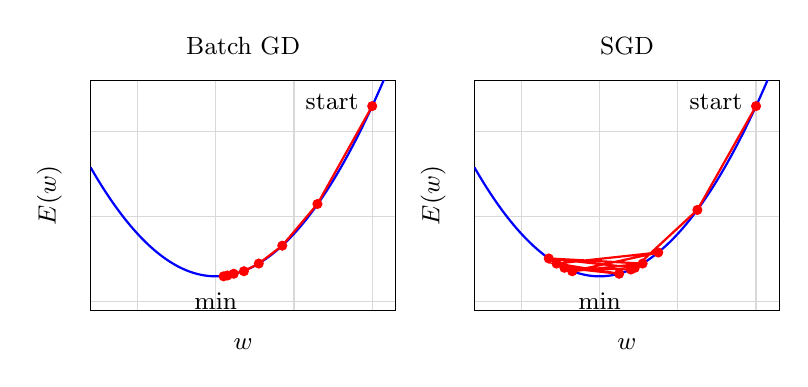
\begin{tikzpicture}
\begin{axis}[
    name=batch, title={\small Batch GD},
    width=0.45\linewidth, height=4.5cm,
    xmin=-1.6, xmax=2.3, ymin=-0.1, ymax=2.6,
    enlargelimits=false,
    grid=major, grid style={gray!30}, major tick length=0pt,
    xlabel={$w$}, ylabel={$E(w)$},
    tick label style={font=\small}, label style={font=\small},
    xticklabels={}, yticklabels={}
]
\addplot[thick, blue, domain=-1.6:2.3, samples=100] {0.5*x^2 + 0.3};
\addplot[red, thick, mark=*, mark size=1.4pt] coordinates {
    (2.00,2.30) (1.30,1.15) (0.85,0.66) (0.55,0.45) (0.36,0.36) (0.23,0.33) (0.15,0.31) (0.10,0.30)
};
\node[font=\small, anchor=east] at (axis cs:1.95,2.35) {start};
\node[font=\small, anchor=north] at (axis cs:0,0.22) {min};
\end{axis}
\begin{axis}[
    at={(batch.east)}, anchor=west, xshift=1cm,
    title={\small SGD},
    width=0.45\linewidth, height=4.5cm,
    xmin=-1.6, xmax=2.3, ymin=-0.1, ymax=2.6,
    enlargelimits=false,
    grid=major, grid style={gray!30}, major tick length=0pt,
    xlabel={$w$}, ylabel={$E(w)$},
    tick label style={font=\small}, label style={font=\small},
    xticklabels={}, yticklabels={}
]
\addplot[thick, blue, domain=-1.6:2.3, samples=100] {0.5*x^2 + 0.3};
\addplot[red, thick, mark=*, mark size=1.4pt] coordinates {
    (2.00,2.30) (1.25,1.08) (0.45,0.40) (-0.65,0.51) (0.55,0.45) (-0.35,0.36) (0.75,0.58) (-0.55,0.45) (0.25,0.33) (-0.45,0.40) (0.40,0.38)
};
\node[font=\small, anchor=east] at (axis cs:1.95,2.35) {start};
\node[font=\small, anchor=north] at (axis cs:0,0.22) {min};
\end{axis}
\end{tikzpicture}
\par}

Each step fits one example, so the path is \textbf{noisy}: downhill on average, but it never fully converges and keeps bouncing near the minimum. \textbf{Slowly decreasing the learning rate} helps it settle. The payoff is that each step is \emph{much} cheaper, so use SGD on large datasets and batch GD on small ones.

\textbf{Update rule.} Loop over $n = 1, \dots, N$; for each $n$, update every $d$:
\[
w_d := w_d - \eta \,
\underbrace{\big(y(\mathbf{x}_n,\mathbf{w}) - t_n\big)}_{\text{error on example } n}\,
\underbrace{x_{n,d}}_{\text{feature } d}
\]
\begin{itemize}
  \item Same as batch GD, but with the $\sum_{n=1}^{N}$ \textbf{dropped}: one example per step.
  \item \textbf{Mini-batch}: use a small batch of $B$ examples per step (e.g.\ 100). $B = 1$ is SGD, $B = N$ is batch GD.
\end{itemize}
